\input{preamble.tex}

\title{Лабораторная работа № 14. \\ Статическая маршрутизация в Интернете. Настройка}
\author{Сущенко Алина Николаевна \\ НПИбд-01-23}
\institute{Российский университет дружбы народов имени Патриса Лумумбы}
\date{2026}

\begin{document}

\frame{\titlepage}

\begin{frame}
\frametitle{Цель работы}
\begin{itemize}
\item Настроить взаимодействие через сеть провайдера посредством статической маршрутизации локальной сети организации с сетью основного здания, расположенного в 42-м квартале в Москве, и сетью филиала, расположенного в г. Сочи.
\end{itemize}
\end{frame}

\begin{frame}
\frametitle{Настройка связи между площадками}

\includegraphics[width=0.8\textwidth]{../images/01.png}
\captionof{figure}{Настройка интерфейсов коммутатора ansusenko-sw-1.}
\end{frame}

\begin{frame}
\frametitle{Настройка связи между площадками}

\includegraphics[width=0.8\textwidth]{../images/02.png}
\captionof{figure}{Настройка интерфейсов маршрутизатора msk-ansusenko-gw-1.}
\end{frame}

\begin{frame}
\frametitle{Настройка связи между площадками}

\includegraphics[width=0.8\textwidth]{../images/03.png}
\captionof{figure}{Настройка интерфейсов маршрутизатора ansusenko-q42-gw-1.}
\end{frame}

\begin{frame}
\frametitle{Настройка связи между площадками}

\includegraphics[width=0.8\textwidth]{../images/04.png}
\captionof{figure}{Настройка интерфейсов коммутатора sch-ansusenko-sw-1.}
\end{frame}

\begin{frame}
\frametitle{Настройка связи между площадками}

\includegraphics[width=0.8\textwidth]{../images/05.png}
\captionof{figure}{Настройка интерфейсов маршрутизатора sch-ansusenko-gw-1.}
\end{frame}

\begin{frame}
\frametitle{Настройка площадки 42-го квартала}

\includegraphics[width=0.8\textwidth]{../images/06.png}
\captionof{figure}{Настройка интерфейсов маршрутизатора ansusenko-q42-gw-1.}
\end{frame}

\begin{frame}
\frametitle{Настройка площадки 42-го квартала}

\includegraphics[width=0.8\textwidth]{../images/07.png}
\captionof{figure}{Настройка интерфейсов коммутатора ansusenko-q42-sw-1.}
\end{frame}

\begin{frame}
\frametitle{Настройка площадки 42-го квартала}

\includegraphics[width=0.8\textwidth]{../images/08.png}
\captionof{figure}{Настройка интерфейсов маршрутизирующего коммутатора ansusenko-hostel-gw-1.}
\end{frame}

\begin{frame}
\frametitle{Настройка площадки 42-го квартала}

\includegraphics[width=0.8\textwidth]{../images/09.png}
\captionof{figure}{Настройка интерфейсов коммутатора ansusenko-hostel-sw-1.}
\end{frame}

\begin{frame}
\frametitle{Настройка площадки в Сочи}

\includegraphics[width=0.8\textwidth]{../images/10.png}
\captionof{figure}{Настройка интерфейсов маршрутизатора sch-ansusenko-gw-1.}
\end{frame}

\begin{frame}
\frametitle{Настройка площадки в Сочи}

\includegraphics[width=0.8\textwidth]{../images/11.png}
\captionof{figure}{Настройка интерфейсов коммутатора sch-ansusenko-sw-1.}
\end{frame}

\begin{frame}
\frametitle{Настройка статической маршрутизации между площадками}

\includegraphics[width=0.8\textwidth]{../images/12.png}
\captionof{figure}{Настройка маршрутизации на msk-ansusenko-gw-1.}
\end{frame}

\begin{frame}
\frametitle{Настройка статической маршрутизации между площадками}

\includegraphics[width=0.8\textwidth]{../images/13.png}
\captionof{figure}{Настройка маршрута по умолчанию на ansusenko-q42-gw-1.}
\end{frame}

\begin{frame}
\frametitle{Настройка статической маршрутизации между площадками}

\includegraphics[width=0.8\textwidth]{../images/14.png}
\captionof{figure}{Настройка маршрута по умолчанию на sch-ansusenko-gw-1.}
\end{frame}

\begin{frame}
\frametitle{Настройка маршрутизации на 42 квартале}

\includegraphics[width=0.8\textwidth]{../images/15.png}
\captionof{figure}{Настройка маршрута до сети общежития.}
\end{frame}

\begin{frame}
\frametitle{Настройка маршрутизации на 42 квартале}

\includegraphics[width=0.8\textwidth]{../images/16.png}
\captionof{figure}{Настройка маршрутизации на ansusenko-hostel-gw-1.}
\end{frame}

\begin{frame}
\frametitle{Настройка NAT на маршрутизаторе msk-ansusenko-gw-1}

\includegraphics[width=0.8\textwidth]{../images/17.png}
\captionof{figure}{Настройка NAT на маршрутизаторе msk-ansusenko-gw-1.}
\end{frame}

\begin{frame}
\frametitle{Проверка корректности настроек}

\includegraphics[width=0.8\textwidth]{../images/18.png}
\captionof{figure}{Результат настроек на ansusenko-q42-sw-1.}
\end{frame}

\begin{frame}
\frametitle{Проверка корректности настроек}

\includegraphics[width=0.8\textwidth]{../images/19.png}
\captionof{figure}{Результат настроек на ansusenko-hostel-sw-1.}
\end{frame}

\begin{frame}
\frametitle{Проверка корректности настроек}

\includegraphics[width=0.8\textwidth]{../images/20.png}
\captionof{figure}{Результат настроек на sch-ansusenko-sw-1.}
\end{frame}

\begin{frame}
\frametitle{Проверка состояния интерфейсов}

\includegraphics[width=0.8\textwidth]{../images/21.png}
\captionof{figure}{show ip interface brief на ansusenko-q42-gw-1.}
\end{frame}

\begin{frame}
\frametitle{Проверка состояния интерфейсов}

\includegraphics[width=0.8\textwidth]{../images/22.png}
\captionof{figure}{show ip interface brief на sch-ansusenko-gw-1.}
\end{frame}

\begin{frame}
\frametitle{Проверка VLAN}

\includegraphics[width=0.8\textwidth]{../images/23.png}
\captionof{figure}{show vlan brief на ansusenko-sw-1.}
\end{frame}

\begin{frame}
\frametitle{Проверка VLAN}

\includegraphics[width=0.8\textwidth]{../images/25.png}
\captionof{figure}{show vlan brief на sch-ansusenko-sw-1.}
\end{frame}

\begin{frame}
\frametitle{Проверка NAT}
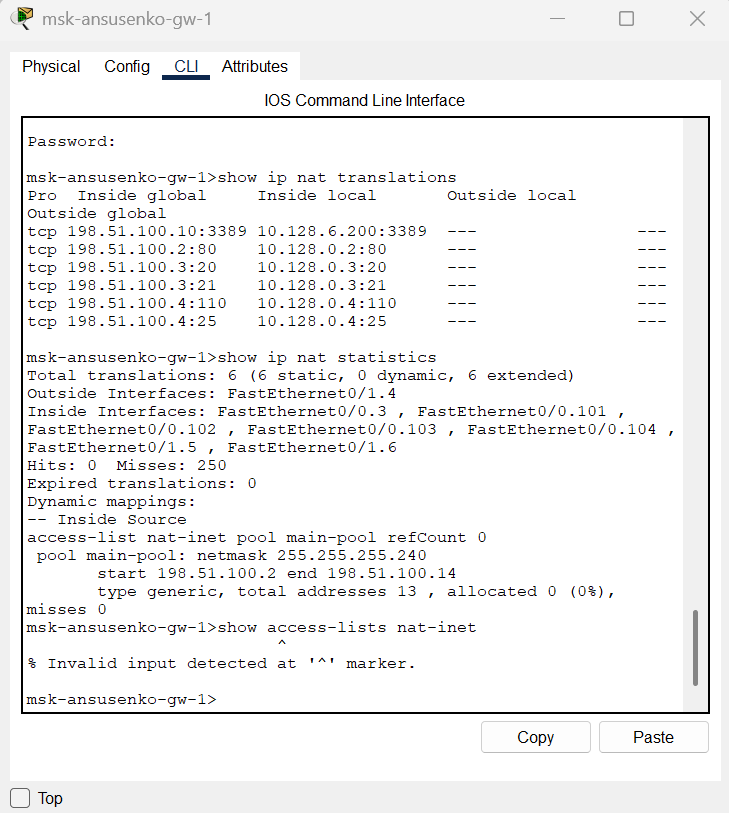
\includegraphics[width=0.8\textwidth]{../images/26.png}
\captionof{figure}{show ip nat translations и show ip nat statistics.}
\end{frame}

\begin{frame}
\frametitle{Ответы на контрольные вопросы}
\begin{enumerate}
\item \textbf{Пример настройки статической маршрутизации между двумя подсетями организации:}
\begin{verbatim}
ip route 192.168.2.0 255.255.255.0 192.168.1.2
ip route 192.168.3.0 255.255.255.0 192.168.1.2
\end{verbatim}
\end{enumerate}
\end{frame}

\begin{frame}
\frametitle{Ответы на контрольные вопросы}
\begin{enumerate}
\setcounter{enumi}{1}
\item \textbf{Процесс обращения устройства из одного VLAN к устройству из другого VLAN:}
\begin{itemize}
    \item Устройство-источник отправляет ARP-запрос на шлюз по умолчанию
    \item Пакет передается на маршрутизатор (или L3-коммутатор)
    \item Маршрутизатор проверяет таблицу маршрутизации и определяет исходящий интерфейс
    \item Маршрутизатор отправляет ARP-запрос в целевом VLAN
    \item После получения MAC-адреса пакет инкапсулируется и отправляется устройству-назначения
\end{itemize}
\end{enumerate}
\end{frame}

\begin{frame}
\frametitle{Ответы на контрольные вопросы}
\begin{enumerate}
\setcounter{enumi}{2}
\item \textbf{Как проверить работоспособность маршрута?}
\begin{verbatim}
ping <IP-адрес назначения>
traceroute <IP-адрес назначения>
show ip route <IP-адрес>
\end{verbatim}
\end{enumerate}
\end{frame}

\begin{frame}
\frametitle{Ответы на контрольные вопросы}
\begin{enumerate}
\setcounter{enumi}{3}
\item \textbf{Как посмотреть таблицу маршрутизации?}
\begin{verbatim}
show ip route           # полная таблица
show ip route static    # только статические маршруты
show ip route connected # только подключенные сети
\end{verbatim}
\end{enumerate}
\end{frame}

\begin{frame}
\frametitle{Выводы}
\begin{itemize}
    \item В ходе выполнения лабораторной работы настроена статическая маршрутизация между тремя площадками (провайдер, 42-й квартал в Москве, филиал в Сочи) с использованием технологии VLAN и subinterface-ов. На маршрутизаторах настроены статические маршруты, включая маршруты по умолчанию и суммарные маршруты. На маршрутизаторе msk-ansusenko-gw-1 выполнена настройка NAT для трансляции адресов внутренних хостов.
    
\end{itemize}
\end{frame}

\end{document}
